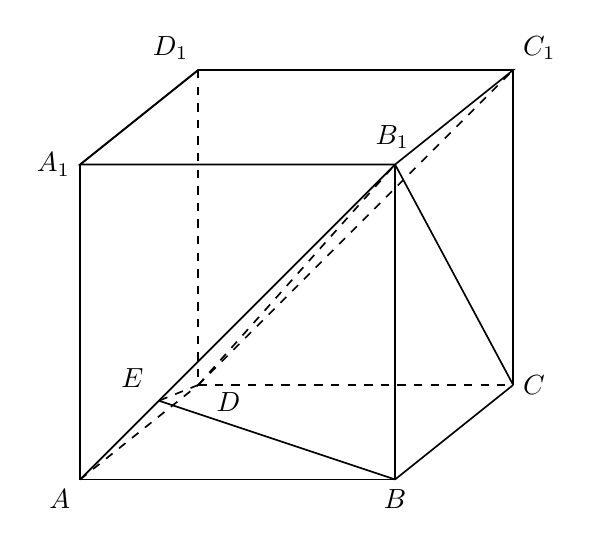
\begin{tikzpicture}[line width=0.6pt, font=\normalsize]
\coordinate (A) at (0,0);
\coordinate (B) at (4,0);
\coordinate (B1) at (4,4);
\coordinate (A1) at (0,4);
\coordinate (D) at (1.5000000000,1.2000000000);
\coordinate (C) at (5.5000000000,1.2000000000);
\coordinate (D1) at (1.5000000000,5.2000000000);
\coordinate (C1) at (5.5000000000,5.2000000000);
\coordinate (E) at (1.0000000000,1.0000000000);
% front face
\draw (A) -- (B) -- (B1) -- (A1) -- cycle;
% top face
\draw (A1) -- (B1) -- (C1) -- (D1) -- cycle;
% verticals / depth
\draw (B) -- (C);
\draw (C) -- (C1);
\draw (A1) -- (D1);
\draw[dashed] (A) -- (D);
\draw[dashed] (D) -- (C);
\draw[dashed] (D1) -- (D);
% diagonals per original: A-C1, A-B1, B1-C, D-B, D-B1

\draw (A) -- (B1);
\draw (B1) -- (C);

\draw[dashed] (D) -- (B1);
\node[below left] at (A) {$A$};
\node[below] at (B) {$B$};
\node[right] at (C) {$C$};
\node[below right=2pt,xshift=1pt,yshift=3pt] at (D) {$D$};
\node[left] at (A1) {$A_{1}$};
\node[above,xshift=-1.0pt,yshift=2pt] at (B1) {$B_{1}$};
\node[above right] at (C1) {$C_{1}$};
\node[above left] at (D1) {$D_{1}$};
\node[above left, xshift=-2pt,yshift=1.0pt] at (E) {$E$};
\draw[dashed] (D)--(C1);\draw[dashed] (D)--(E);\draw (E)--(B);
\end{tikzpicture}
